\documentclass[%
%  reprint,
superscriptaddress,
% groupedaddress,
%unsortedaddress,
%runinaddress,
%frontmatterverbose, 
% preprint,
% preprintnumbers,
nofootinbib,
%nobibnotes,
%bibnotes,
 amsmath,amssymb,
 aps,
%pra,
%prb,
%rmp,
%prstab,
%prstper,
%floatfix,
showkeys
]{revtex4-2}
\usepackage[utf8]{inputenc}
\usepackage{graphicx}% Include figure files
\usepackage{dcolumn}% Align table columns on decimal point
\usepackage{bm}% bold math
\usepackage{hyperref}
\usepackage[bottom]{footmisc}
\usepackage{footnote}
\usepackage{cleveref}

\begin{document}
\title{ATHENA - neutron DVCS with spectator tagging in deuteron}

\author{Zhoudunming~Tu}
\email{zhoudunming@bnl.gov}
\affiliation{%
 Department of Physics, Brookhaven National Laboratory, Upton, NY 11973, USA
}

\author{Salvatore~Fazio}
\email{salvatore.fazio@unical.it}
\affiliation{%
 University of Calabria \& INFN-Cosenza, Italy
}

%\date{Nov 2021}
\maketitle

Partonic imagining is one of the most important scientific goals of the Electron-Ion Collider, where most of the experimental endeavors are based on measurement using a proton. For example, Deeply Virtual Compton Scattering (DVCS) on a proton, is one of the golden channels to study the GPDs of quarks and is sensitive to gluons via evolution. However, there are further questions on GPDs that cannot be answered by only using a proton, e.g., quark-flavor separation, nuclear GPDs, and connections to the short-range nuclear correlations. Hereby, we propose to study the GPDs of a neutron by measuring DVCS on an incoherent electron-deuteron ($e+d$) scattering, with both outgoing nucleon (active neutron and spectator proton) tagged in the experiment. 

The advantages of using deuteron beam is the following: (i) theoretical understanding of the deuteron is clear and most studied; (ii) by tagging a spectator proton and measure its momentum distribution, we can either go to essentially zero momentum for a free neutron or go to high momentum tail to study modifications. Similar proposals have been made to measure a free neutron structure using a similar technique~\cite{Jentsch:2021qdp}.

In Fig.~\ref{fig:figure_1} left, the momentum transfer $|t|$ distribution of DVCS process on a neutron is shown, where the tagged spectator proton momentum distribution in the ion rest frame is shown on the Fig.~\ref{fig:figure_1} right. Due to the fermi momentum of nucleons in deuteron, the standard reconstruction of $|t|$ using scattered neutron would not work since the initial momentum is unknown event-by-event. Therefore, we propose to use an alternative method on measuring the $|t|$, which is to use the spectator proton to obtain the information of the initial neutron momentum. Therefore, $|t| = - (n'-n)^{2}$, where $n$ is obtained thru the measurement of proton spectator four momentum. 

In Fig.~\ref{fig:figure_1} left, the histogram is the generated level neutron $|t|$ distribution, where the markers represent the fully reconstructed $|t|$ using the ATHENA detectors. The acceptance in $|t|$ is roughly 80-90\% at low $|t|$, while the loss at higher value is mostly due to the loss in tagging the active neutron in ZDC. Alternatively, the $|t|$ measurement could be done using the four momentum of the scattered electron and the photon, where a higher acceptance at higher $|t|$ can be achieved. 


\begin{figure}[thb]
\centering
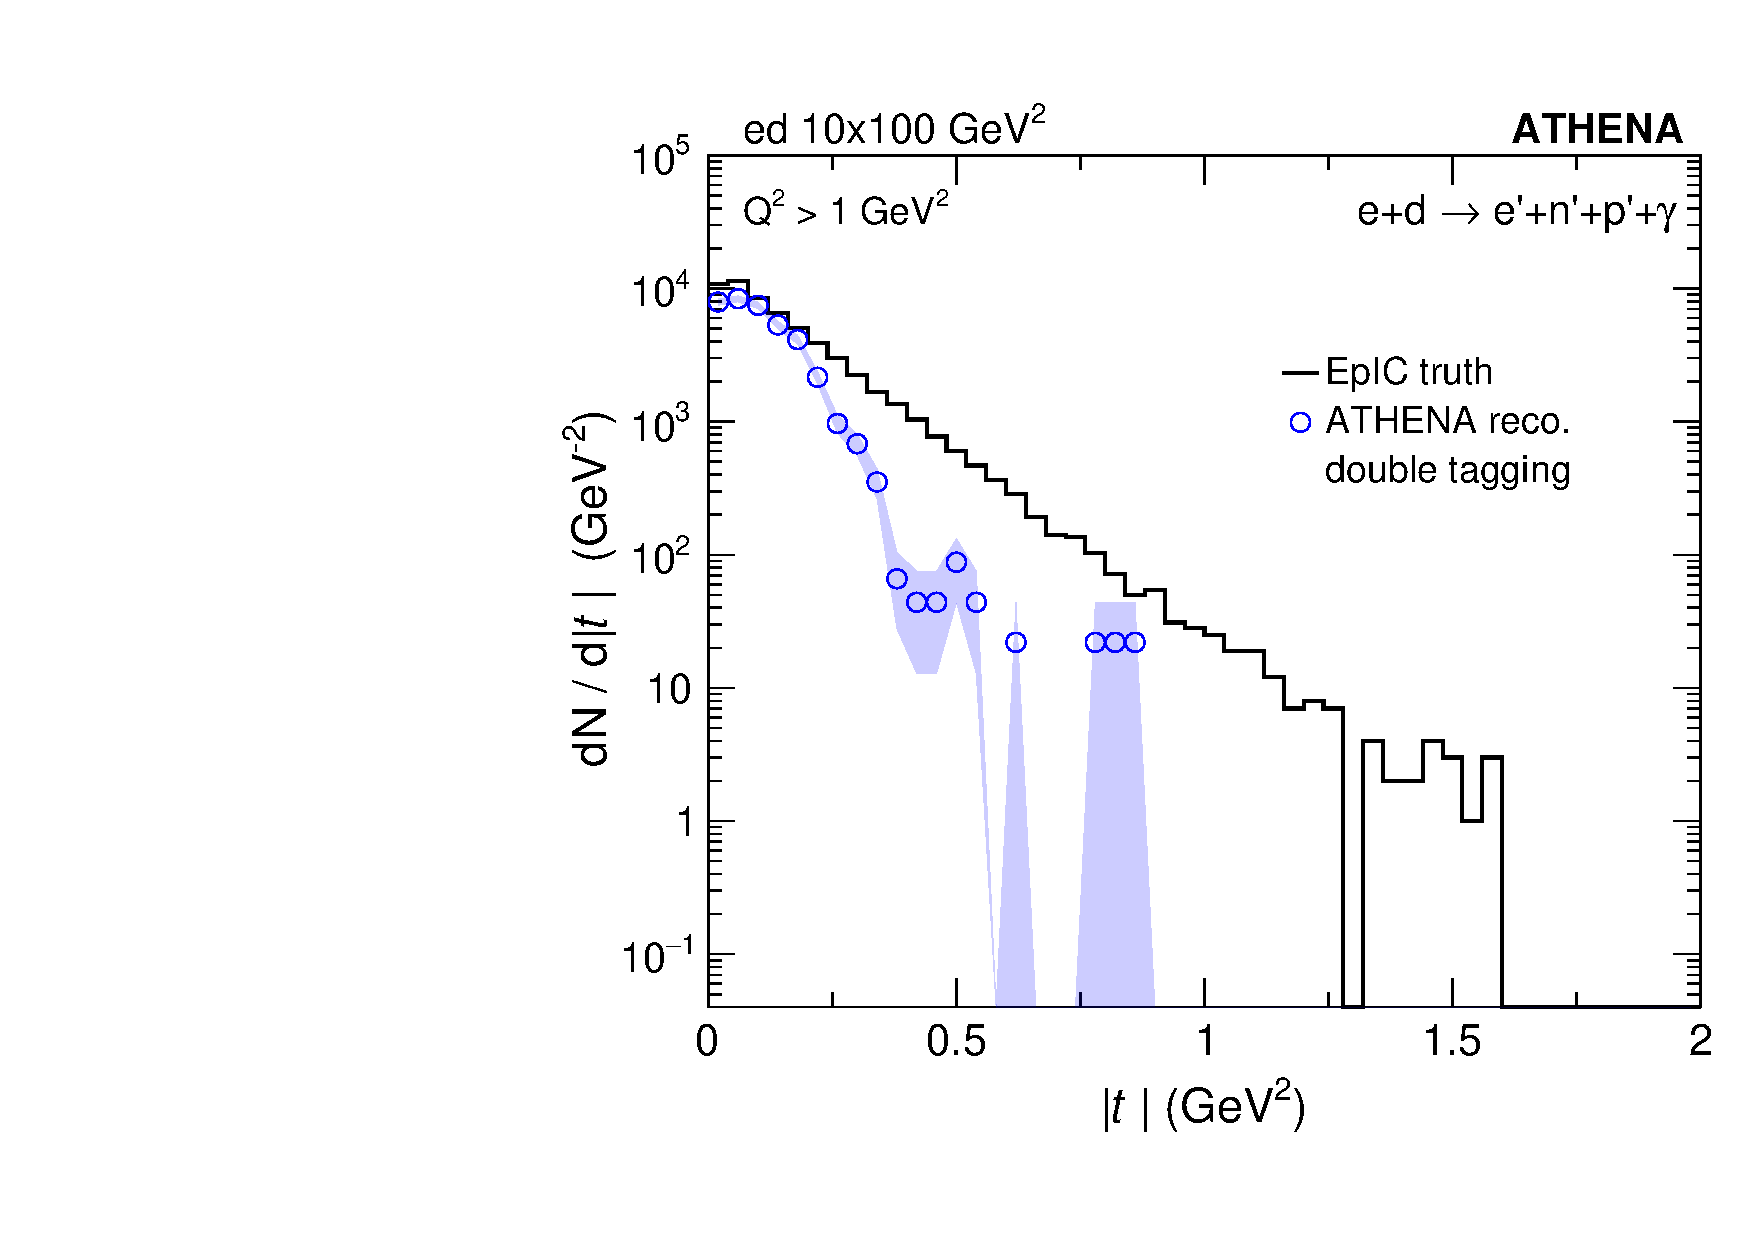
\includegraphics[width=3.5in]{Figure_1.pdf}
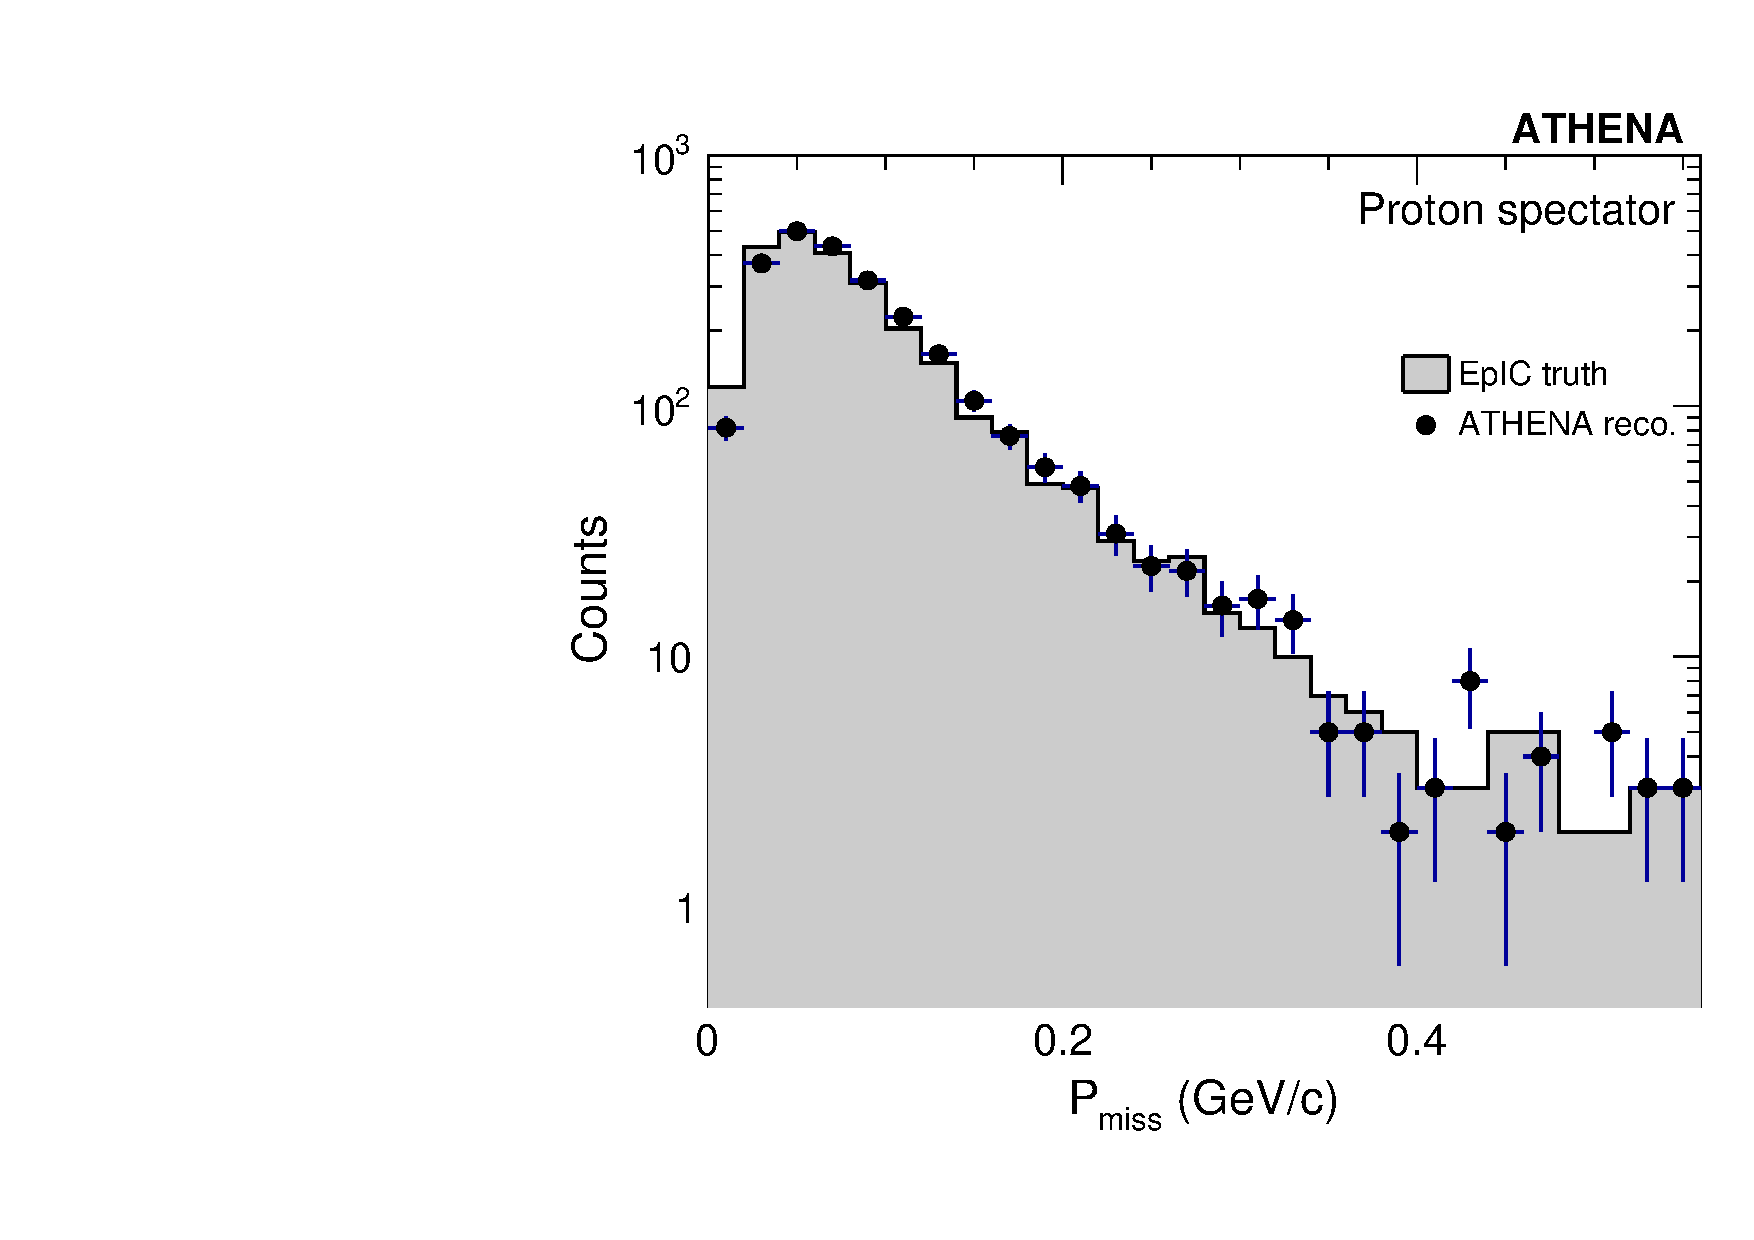
\includegraphics[width=3.5in]{Figure_2.pdf}
  \caption{ \label{fig:figure_1} Momentum transfer $|t|$ distribution in DVCS on a neutron with proton spectator tagged in $ed$ collisions. Both generated and reconstructed $|t|$ distributions are shown, where the momentum distribution of spectator proton in the ion rest frame is also shown. }
\end{figure}

\bibliography{reference}

\end{document}